%% Based on a TeXnicCenter-Template by Gyorgy SZEIDL.
%%%%%%%%%%%%%%%%%%%%%%%%%%%%%%%%%%%%%%%%%%%%%%%%%%%%%%%%%%%%%

%------------------------------------------------------------
%
\documentclass[a4paper]{article}%
%Options -- Point size:  10pt (default), 11pt, 12pt
%        -- Paper size:  letterpaper (default), a4paper, a5paper, b5paper
%                        legalpaper, executivepaper
%        -- Orientation  (portrait is the default)
%                        landscape
%        -- Print size:  oneside (default), twoside
%        -- Quality      final(default), draft
%        -- Title page   notitlepage, titlepage(default)
%        -- Columns      onecolumn(default), twocolumn
%        -- Equation numbering (equation numbers on the right is the default)
%                        leqno
%        -- Displayed equations (centered is the default)
%                        fleqn (equations start at the same distance from the right side)
%        -- Open bibliography style (closed is the default)
%                        openbib
% For instance the command
%           \documentclass[a4paper,12pt,leqno]{article}
% ensures that the paper size is a4, the fonts are typeset at the size 12p
% and the equation numbers are on the left side
%
\usepackage{amsmath}%
\usepackage{amsfonts}%
\usepackage{amssymb}%
\usepackage{graphicx}

\usepackage[utf8]{inputenc}
\usepackage[T1]{fontenc}
\usepackage[francais]{babel}
\usepackage{float}
%\usepackage[pdftex]{graphicx}


%-------------------------------------------

\newcommand{\HRule}{\rule{\linewidth}{0.5mm}}

\begin{document}

\begin{titlepage}
\begin{center}

% Upper part of the page. The '~' is needed because \\
% only works if a paragraph has started.

\textsc{\LARGE INSA Rennes}\\[1.5cm]

\textsc{\Large Jeu Small World}\\[0.5cm]

% Title
\HRule \\[0.4cm]
{ \huge \bfseries Rapport de conception \\[0.4cm] }

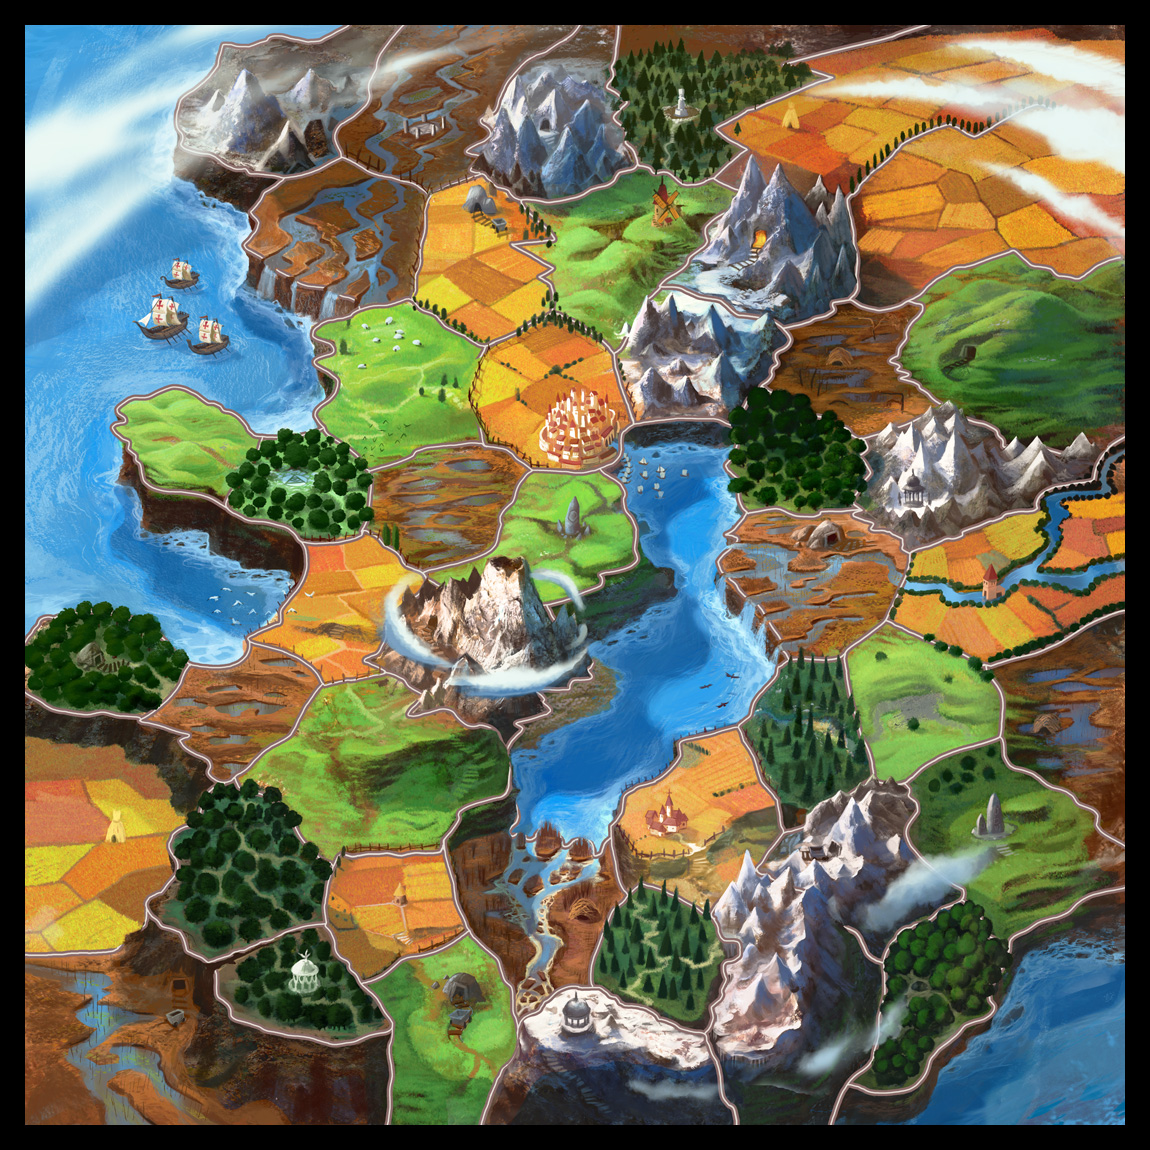
\includegraphics[width=0.8\textwidth]{./images/plateau_smallworld.jpg}~\\[1cm]


\HRule \\[1.5cm]

% Author and supervisor
\begin{minipage}{0.4\textwidth}
\begin{flushleft} \large
\emph{Auteurs :}\\
Damien \textsc{Crémilleux}
Lauriane \textsc{Holy}
\end{flushleft}
\end{minipage}

\vfill

\end{center}
\end{titlepage}

\newpage
\setcounter{page}{2}
~
\newpage

\tableofcontents

\newpage
~
\newpage

\section*{Introduction}
\addcontentsline{toc}{section}{Introduction}

Le projet de conception et de programmation orienté objet a pour objectif de concevoir un jeu inspiré de Small World, un jeu de stratégie au tour par tour où chaque joueur dirige un peuple. Les joueurs bouge ses unités sur une carte et peux combattre celles de son adversaire. Le but est d'obtenir plus de points que les autres peuples.

\medskip

Ce rapport traite les thèmes essentiels aborder lors de la phase d'analyse et de conception du jeu. Son plan est fortement inspiré du polycopié d'énoncé. L'énoncé du projet est repris dans ce rapport afin de faire le parallèle entre les tâches à réaliser et notre modélisation. 

\medskip

Ainsi, les principes et les règles du jeux Small World sont d'abord rappelés, afin de comprendre et de cerner les  différents cas d'utilisations. Les déroulement de cas d'activités (comme par exemple un tour de jeu) sont explicités à l'aide de diagramme de cas d'activité.
La deuxième partie montre la modélisation suivant les diagrammes de séquence et de classes qui découlent de la première partie.


\section{Principes et utilisation}

Comme énoncé dans l'introduction Small World est un jeu tour-par-tour où chaque joueur dirige un peuple. Le but du jeu est de gérer des unités sur une carte pour obtenir le plus de points possible à la fin d’un certain nombre de tours. Le placement de chaque unité rapporte plus ou moins de points. Les unités d’un joueur peuvent également attaquer les unités d’un autre joueur pour détruire des unités (limitant ainsi l’acquisition de points de l’adversaire) et occuper une case de la carte. Les points sont comptés à la fin de la partie, c.-à-d. après un nombre prédéfini de tours. Le jeu se déroule sur une carte du monde sur laquelle les unités se déplacent.

\subsection{Règles du jeux}
\subsubsection{Les peuples}
Il existe trois peuples, Gaulois, Viking et Nain, ayant des caractéristiques très différentes influant sur les stratégies de jeu :

\begin{itemize}

\item Gaulois. \begin{itemize}
\item Le coût de déplacement sur une case Plaine est divisé par deux.
\item Une unité Gauloise fournit 1 point de plus lorsqu’elle occupe une case du type plaine.
\item Une unité Gauloise n’acquière aucun point sur les cases de type montagne.
\end{itemize}
\item Vikings. \begin{itemize}
\item L’unité Viking a la capacité de se déplacer sur l’eau. L’occupation d’une case eau ne rapporte cependant aucun point.
\item Une unité Viking fournit 1 point de plus lorsqu’elle occupe une case au bord de l’eau.
\item Une unité Viking n’acquière aucun point sur les cases de type désert.
\end{itemize}
\item Nains. \begin{itemize}
\item Lorsqu’elle se trouve sur une case montagne, une unité Nain a la capacité de se déplacer sur n’importe quelle case montage de la carte à condition qu’elle ne soit pas occupée par une unité adverse.
\item Une unité Nain fournit 1 point de plus lorsqu’elle occupe une case forêt.
\item Une unité Nain n’acquière aucun point sur les cases de type plaine.
\end{itemize}
\end{itemize}


À chaque tour, toutes unités peuvent être déplacées ou attaquer. Par défaut (c.-à-d. hors bonus), chaque unité peut se déplacer d’une case par tour. Chaque unité possède 2 d’attaque, 1 de défense et 2 points de vie.

\subsubsection{La Carte du Monde}
La carte du monde se compose de cases carrées. La largeur d’une case est de 50 pixels. Il existe différents types de case : montagne, plaine, désert, eau, forêt. La carte sera créée en début de partie de manière aléatoire.

Il existe 3 types de cartes :
\begin{itemize}
\item Démo : 2 joueurs, 5 cases x 5 cases, 5 tours, 4 unités par peuples.
\item Petite : 2 joueurs, 10 cases x 10 cases, 20 tours, 6 unités par peuples.
\item Normale : 2 joueurs, 15 cases x 15 cases, 30 tours, 8 unités par peuples.
\end{itemize}

\subsubsection{Les Combats}
Pour qu’une unité puisse lancer une attaque contre une unité d’un autre peuple, elles doivent se situées sur des cases juxtaposées (attaque en diagonale impossible cependant). Lorsqu’une unité attaque une case contenant plusieurs unités, la meilleure unité défensive est choisie. Une unité attaquée possédant 0 en défense meurt immédiatement. Sinon, un certain nombre de combats a lieu. Ce nombre est choisi aléatoirement à l’engagement (entre 3 et le nombre de points de vie de l’unité ayant le plus de points de vie + 2 points). Le combat s’arrête lorsque ce nombre est atteint ou lorsque l’une ou autre des unités n’a plus de vie. Chaque combat calcul les probabilités de perte d’une vie de l’attaquant. Par exemple, Si l’attaquant a 4 en attaque et l’attaqué a 4 en défense (en tenant compte des bonus de terrain et du nombre de points de vie restant), l’attaquant à 50\% de (mal-)chance de perdre une vie. S’il a 3 att. contre 4 déf., le rapport de force est de 75\% : 3/4= 25\%, 25\% de 50\% = 12.5\%, 50\%+12.5\%=62.5\% chance pour l’attaquant de perdre une vie.

Explications du calcul : par défaut 2 unités égales ont 50\% de gagner. Puisque dans le cas présent un écart de 25\% est constaté entre les deux unités, il est nécessaire de pondérer le 50\% par ces 25\% ce qui donne 62.5\% contre 37.5\%. S’il a 4 att. contre 2 déf., le taux baisse à 25\% (2/4 = 50\%, 50\% de 50\% = 25\%, 25\%+50\% = 75\% pour l’attaqué, 100\%-75\%=25\% pour l’attaquant). Évidemment, lorsque l’attaquant gagne cela signifie que l’adversaire perd un point de vie. Les points de vie entrent en compte dans le calcul des probabilités : si une unité attaquante ayant 4 en attaque possède 75\% de sa vie, alors son attaque sera au final de 4*75\% = 3. L’unité attaquée suit le même calcul pour sa défense. 

À la fin d’un combat gagné par l’attaquant et si la case du vaincu ne contient plus d’unité, ce dernier se déplace automatiquement sur cette case. Lorsqu’un joueur n’a plus d’unité, il est éliminé. Lorsqu’il ne reste plus qu’un seul joueur dans une partie, celui-ci a gagner. Une unité ne regagne pas ses points de vie d’un tour à un autre.

\subsubsection{La Vue}
La carte, ses ressources, les unités de tous peuples sont visibles par tous les joueurs. Le jeu doit permettre de voir la carte du dessus (vue plateau) contrairement à beaucoup de jeux  
une vue isométrique.

\subsubsection{Début de Partie}
Au début du jeu, chaque joueur choisi son peuple. Chaque peuple débute la partie avec toutes ses unités sur la même case de la carte choisi de manière à ce que les joueurs ne soient pas trop proche. L’ordre de jeu est choisie aléatoirement en début de partie. Les joueurs jouent chacun leur tour sur leur même ordinateur.

\subsubsection{Tour de jeu}
\label{tourdejeu}
Lorsqu’un joueur peut jouer (c.-à-d. une fois par tour), il peut déplacer toutes ses unités suivant leur nombre de déplacements (un déplacement sur une case coûte un point de déplacement). Il est possible pour chaque unité de passer son tour (généralement par le biais de la touche espace). Une unité combattante peut engager un combat s’il lui reste au moins un point de mouvement. Lorsqu’un joueur a fini son tour, il clique sur le bouton correspondant ("Fin tour"). C’est alors au joueur suivant de commencer son tour. La partie se termine lorsque le nombre de tours prédéfini en début de partie à été effectué, ou lorsqu’il ne reste qu’un seul joueur sur le plateau.

\subsection{Cas d'utilisation et leur déroulement}

\subsubsection{Fonctionnalités globales}
Suite à la lecture de ces énoncés, il est possible d'illustrer les fonctionnalités globales de notre jeu Small World, montrées à la Figure~\ref{fig:jeuglobal}.

\begin{figure}[H]
    \centering
    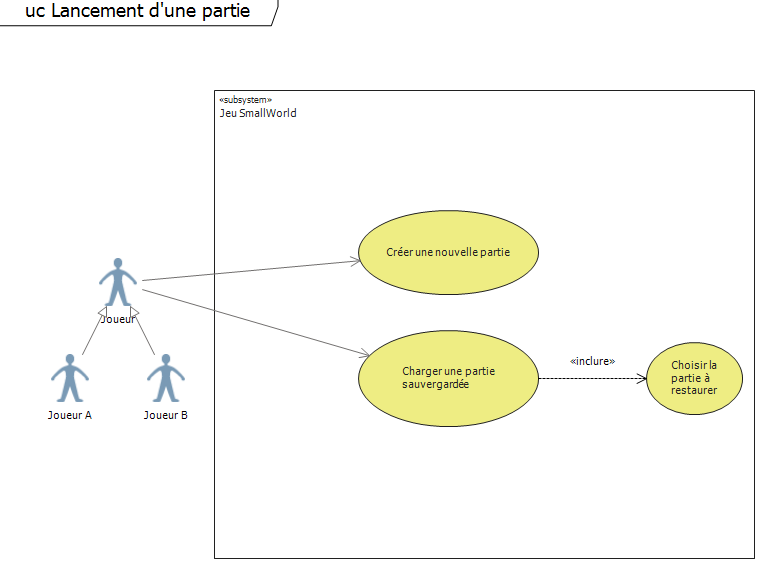
\includegraphics[width=\textwidth]{./images/cas_dutilisation/jeuglobal.png}
		\caption{Diagramme de cas d'utilisation global du jeu Small World}
		\label{fig:jeuglobal}
\end{figure}

\subsubsection{Création d'une partie}

La création d'une partie est illustrée de façon plus précise à la Figure~\ref{fig:cas_creerpartie}.
Lorsque l'on crée une partie, le joueur~A commence par choisir son nom de joueur puis son peuple. Ensuite le joueur~B fait de même et procède au choix de la taille de la carte, avant de lancer la partie. Le joueur~B est donc plus spécialisé que le joueur~A. Cette suite d'interaction est montrée à la Figure~\ref{fig:inter_creerpartie}

\begin{figure}[H]
    \centering
    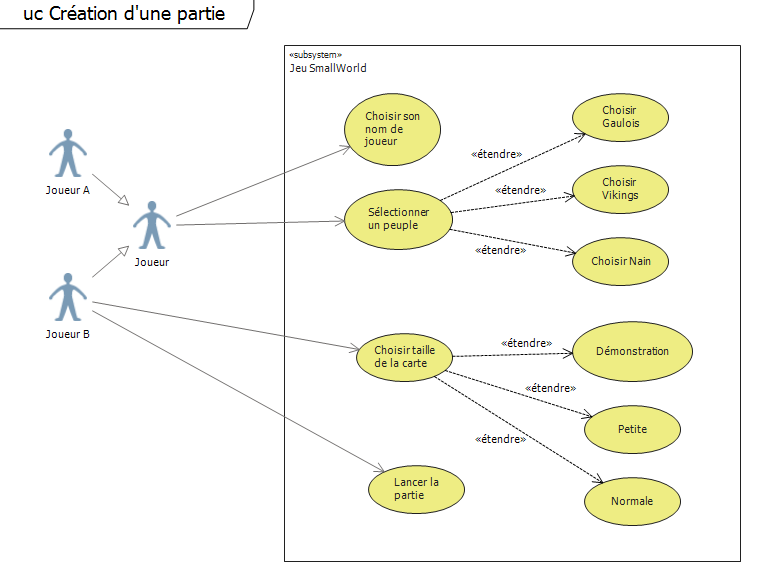
\includegraphics[width=\textwidth]{./images/cas_dutilisation/creerpartie.png}
		\caption{Diagramme de cas d'utilisation de création d'une partie}
		\label{fig:cas_creerpartie}
\end{figure}

\begin{figure}[H]
    \centering
    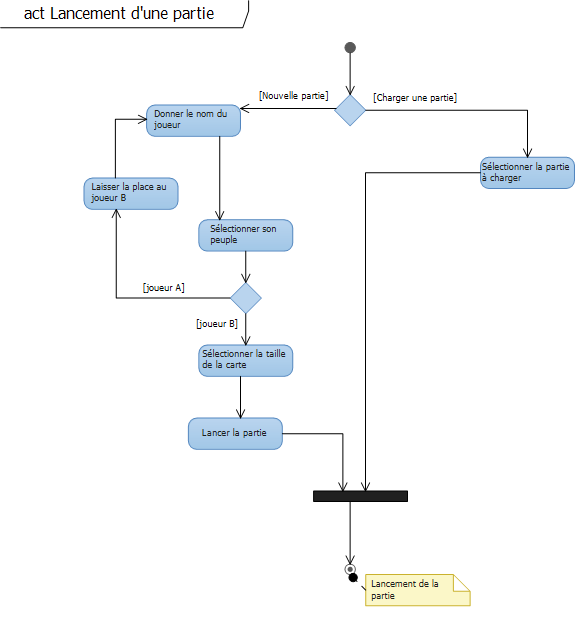
\includegraphics[width=\textwidth]{./images/interaction/creerpartie.png}
		\caption{Diagramme de d'activité de création d'une partie}
		\label{fig:inter_creerpartie}
\end{figure}

\subsubsection{Tour de jeu}
La description d'un tour de jeu, faite à la page~\pageref{tourdejeu}, permet de réaliser le diagramme de cas d'utilisation d'un tour de jeu (Figure~\ref{fig:cas_tourdejeu}). Le déroulement du processsus est représenté sur la Figure~\ref{fig:inter_tourdejeu}.

\begin{figure}[H]
    \centering
    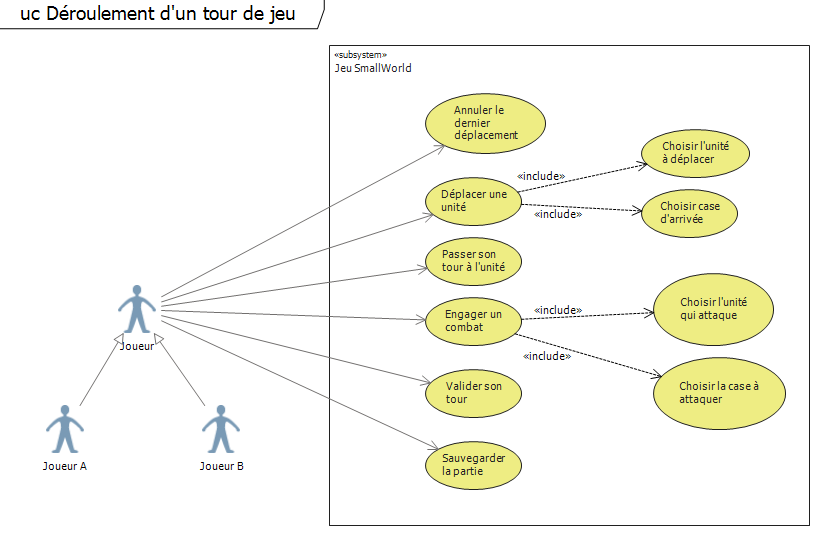
\includegraphics[width=\textwidth]{./images/cas_dutilisation/tourdejeu.png}
		\caption{Diagramme de cas d'utilisation d'un tour de jeu}
		\label{fig:cas_tourdejeu}
\end{figure}

\begin{figure}[H]
    \centering
    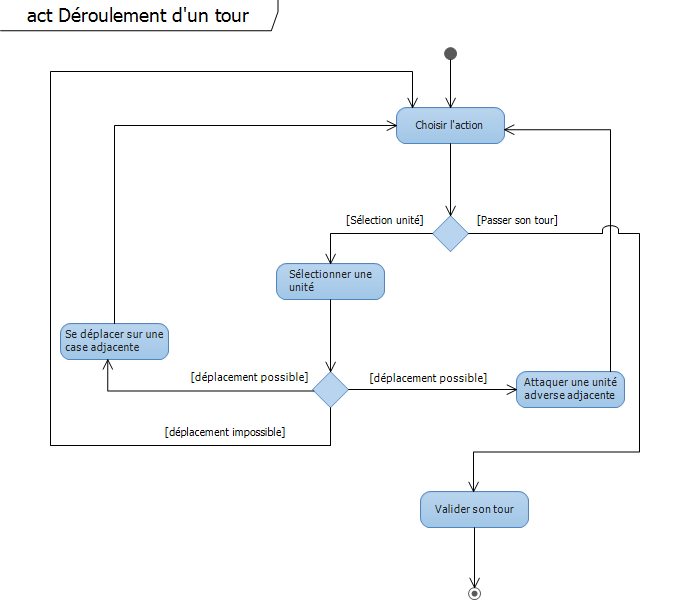
\includegraphics[width=\textwidth]{./images/interaction/tourdejeu.png}
		\caption{Diagramme d'activité d'un tour de jeu}
		\label{fig:inter_tourdejeu}
\end{figure}

\subsubsection{Les combats}
Au cours d'un tour de jeu, le joueur peut décider de combattre le joueur adverse à l'aide de ses unités. Le déroulement d'un combat est montré à l'aide de la Figure~\

\begin{figure}[H]
    \centering
    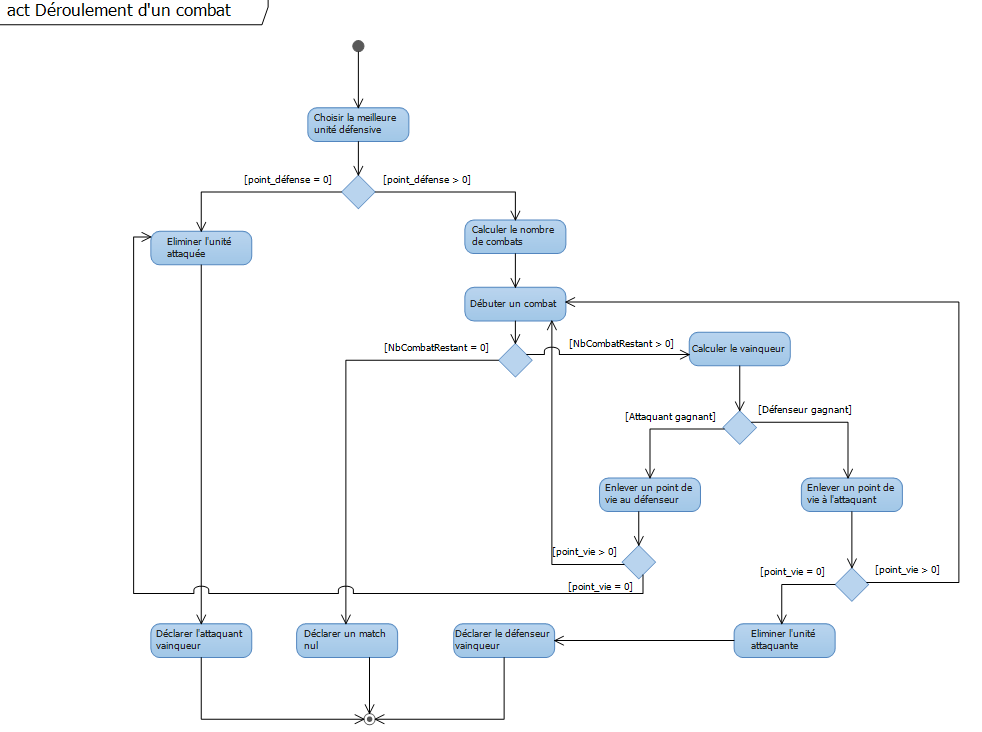
\includegraphics[width=\textwidth]{./images/interaction/combat.png}
		\caption{Diagramme d'activité d'un combat}
		\label{fig:inter_combat}
\end{figure}

\subsubsection{Les unités}

%todo{insérer diagramme d'état transition}

\section{Modélisation}

Les fonctionnalités du jeu étant définies, nous allons maintenant modéliser les différents aspects de celui-ci à l'aide des patrons de conception. Sur les diagrammes de classe qui suivent, les interfaces ne sont pas représentées, seulement les classes qui en dérivent.

\subsection{Création de la partie}

Le patron de conception utilisé est le monteur. L'utilisation de ce patron de conception permet d'extérioriser la création d'une partie, un objet complexe. En outre, le monteur sert à créer plusieurs types de parties. Le monteur est représenté à la Figure~\ref{fig:class_monteur}.

\begin{figure}[H]
    \centering
    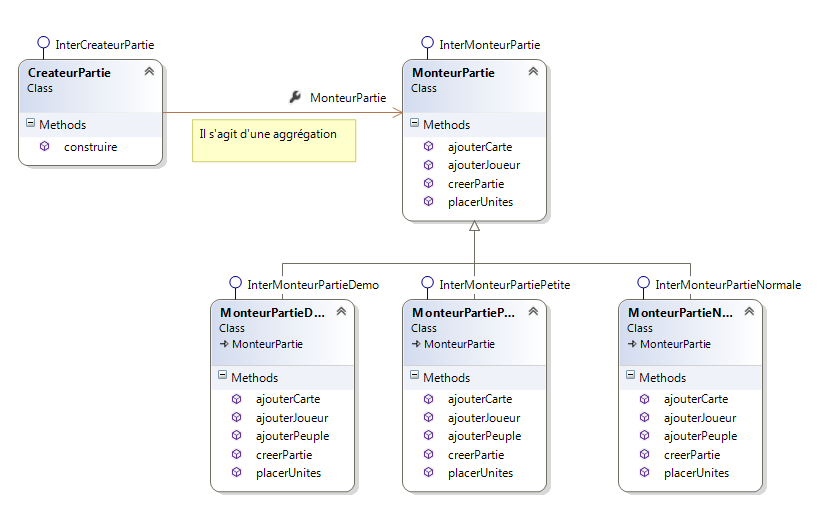
\includegraphics[width=\textwidth]{./images/classe/monteur.png}
		\caption{Diagramme de classe du monteur}
		\label{fig:class_monteur}
\end{figure}


\subsection{Création des différents types de cartes}

Lors de la création d'une partie, les joueurs ont le choix entre trois tailles de cartes : démo, petite ou normale. Différents algorithmes seront développés pour ces tailles. Afin de modéliser ce changement de comportement, c'est-à-dire de changer d'algorithme en fonction du contexte, le patron de conception utilisé est la stratégie. La stratégie est représenté à la Figure~\ref{fig:class_strategie}.

\begin{figure}[H]
    \centering
    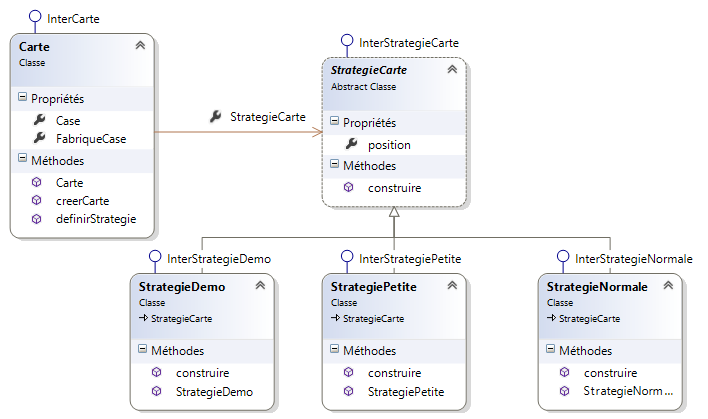
\includegraphics[width=\textwidth]{./images/classe/strategie.png}
		\caption{Diagramme de classe de la stratégie}
		\label{fig:class_strategie}
\end{figure}


\subsection{Modélisation de la carte}

Il existe cinq types de cases dans Small World. Pour ne pas instancier un grands nombres de cas et devenir trop gourmand au niveau de la mémoire, le patron de conception poids-mouche est mis en place. Nous évitons ainsi la création répétée d'une même case. La Figure~\ref{fig:class_poidsmouche} illustre le poids-mouche.

\begin{figure}[H]
    \centering
    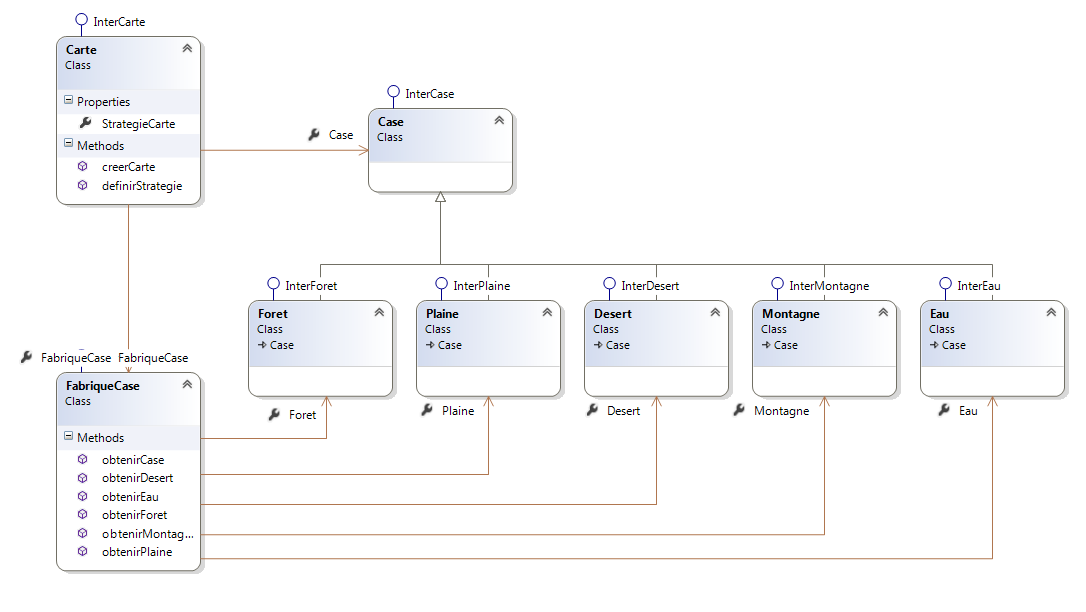
\includegraphics[width=\textwidth]{./images/classe/poidsmouche.png}
		\caption{Diagramme de classe du poids mouche}
		\label{fig:class_poidsmouche}
\end{figure}

\subsection{Gestion des peuples et des unités}

Lors de la création d'une partie, le joueur choisit entre trois peuples. Le jeu devra donc manipuler les unités sans savoir s'il s'agit de vikings, gaulois ou nains. Le patron de conception fabrique est implémenté afin de résoudre ce problème, et de définir une interface pour la création de peuples. En outre, il sera maintenant facile de rajouter un nouveaua peuple.
Les unités étant d'un seul type (il n'y pas d'unité spécialisée au sein d'un peuple), il n'y a pas besoin de fabrique pour les unités. On utilise une classe abstraire pour définir les éléments communs aux unités des différents peuples. Ces éléments sont présentés à la Figure~\ref{fig:class_fabrique}.

\begin{figure}[H]
    \centering
    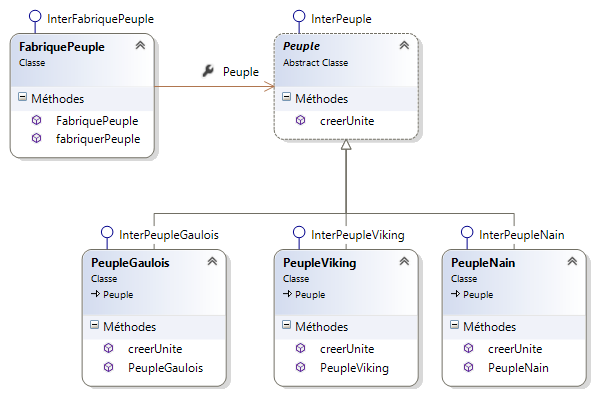
\includegraphics[width=\textwidth]{./images/classe/fabrique.png}
		\caption{Diagramme de classe de la fabrique}
		\label{fig:class_fabrique}
\end{figure}

\newpage

\section*{Conclusion}
\addcontentsline{toc}{section}{Conclusion}

\end{document}
